\chapter{L'état de l'art de la détection de la détérioration visuelle dans le domaine des pixels}
\label{chap-revuelit}
Dans ce chapitre, nous faisons état de la littérature sur les approches de
détection de la détérioration visuelle. Il ne s’agit pas, ici, d’une simple
énumération, mais bien d’une suite logique d’ouvrages permettant de comprendre
l’introduction et l’évolution de plusieurs concepts fondamentaux, sur lesquels
reposent nos contributions.

La détection de la détérioration visuelle sert à identifier la dégradation
visuelle engendrée par le décodage de paquets corrompus. Pour décoder ces
paquets, le décodeur du canal de transmission doit interagir avec le décodeur
vidéo (source) afin d'identifier et de rendre disponible les paquets corrompus.
Ce type d'interaction porte le nom de \textit{Joint Source Channel Decoding}.
Notre prologue, \sect{sect-prologue}, expose les origines du \textit{Joint
Source Channel Decoding}. La \sect{sect-SourceChannel} offre un compte rendu des
notions du \textit{Joint Source Channel Decoding} qui s'appliquent
spécifiquement au transport de séquences vidéos. Les améliorations apportées à
une de ces notions, l'analyse syntaxique, sont présentées à la
\sect{sect-SyntaxeAnalysis}. Finalement, à la \sect{sect-Combined}, les
approches combinant l'analyse syntaxique à la détection de la détérioration
visuelle dans le domaine des pixels sont décrites.

\begin{section}{Prologue}
\label{sect-prologue}
Dans son ouvrage \textit{A Mathematical Theory of Communication},
\citet{Shannon1948} explique sous l'allégorie ingénieuse du télégraphe, la
notion même du \textit{Joint Source Channel Decoding}. L'usage d'un langage
redondant, tel l'anglais, comme encodage pour le télégraphe a l'avantage d'être
résistant aux erreurs du canal de transmission. Le contexte du message permet
la reconstruction des mots, même si plusieurs lettres de ceux-ci sont bruitées
\citep[p.~24]{Shannon1948}.

En \citeyear{Modestino1979}, \citeauthor{Modestino1979} sont les premières
personnes à proposer l'utilisation du \textit{Joint Source Channel Decoding}
pour améliorer le transport d'images numériques. Déjà en 1979,
\citeauthor{Modestino1979} déplorent le gaspillage de la bande passante,
introduit par les stratégies de résilience aux erreurs. Un gaspillage qui, 30
ans plus tard, est toujours présent sur les réseaux sans fil
\citep[p.1]{Duhamel2010}.

\begin{figure}
	\fbox{
		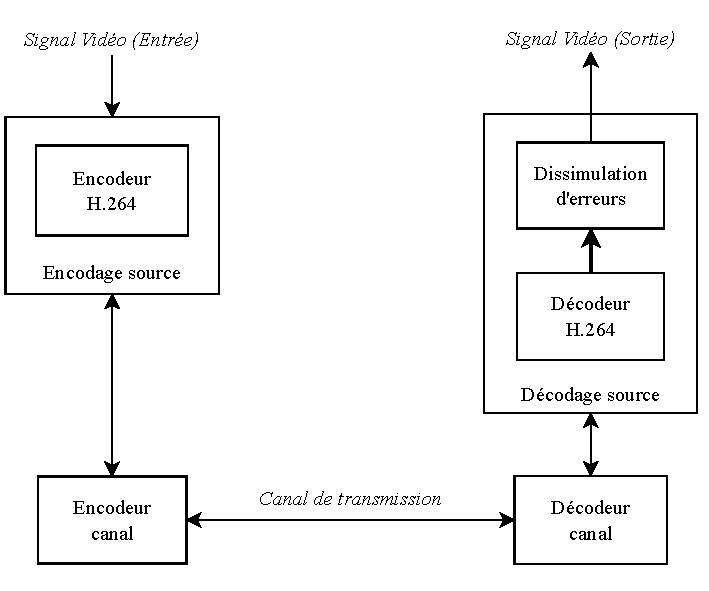
\includegraphics{images/VideoCommunication.pdf}}
	\caption[Composantes liées au transport de séquences vidéos]{Diagramme à blocs
des composantes liées au transport de séquences vidéos. Adaptée de
\citet[p.~976]{Wang1998}}
	\label{fig-VideoCommunication}
\end{figure}

Avant de poursuivre, décrivons les composantes liées au \textit{Joint Source
Channel Decoding}. La \fig{fig-VideoCommunication} résume les étapes et les
interactions du \textit{Joint Source Channel Decoding}. Tout d'abord, l'encodeur
H.264 retire la redondance d'un signal vidéo. Par la suite, l'encodeur du canal
va empaqueter le contenu et insérer les mécanismes de résilience à l'erreur
nécessaires selon le canal de transmission. Notons l'ajout de données
redondantes comme un des mécanismes de résilience à l'erreur. Dès la réception
de paquets chez le destinataire, le décodeur du canal dépaquète ceux-ci et
valide que leur contenu est intact. À l'aide des données dépaquetées, le
décodeur H.264 reconstruit le signal vidéo. Cependant, si des données sont
manquantes ou corrompues, le décodeur H.264 fait appel à un algorithme de
dissimulation d'erreurs pour estimer ces dernières.
\end{section}

\begin{section}{Établir le lien entre le décodeur vidéo et celui du canal de
transmission}
\label{sect-SourceChannel}
Les techniques de résilience aux erreurs sur des réseaux non fiables ont suscité
beaucoup d'intérêt dans les années 1980 et 1990. En \citeyear{Wang1998}, dans
leur revue sur les techniques de contrôle et de dissimulation d'erreurs lors du
transport de séquences vidéos\footnoteETS{Traduction de l'auteur du titre
\textit{Error Control and Concealment for Video Communication: A Review}.}
\citep{Wang1998}, \citeauthor{Wang1998} récapitulent, entre autres, l'état de
l'art, de l'époque, des stratégies de résilience aux erreurs.
\citeauthor{Wang1998} présentent une multitude d'approches. Parmi celles-ci, ils
identifient un type d'approches qu'ils qualifient d'approches de dissimulation
par post-traitement effectué par le décodeur \citep[Chap. 5]{Wang1998}. Ce type
résume, de façon exacte, les approches que nous présentons dans cet ouvrage.
Leurs composantes sont illustrées à la \fig{fig-VideoCommunication}. Parmi les
approches de dissimulation présentées en \citeyear{Wang1998}, on remarque:
\textit{Motion-Compensated Temporal Prediction}~\citep{Ghanbari1993},
\textit{Maximally Smooth Recovery}~\citep{Wang1993}, \textit{Projection onto
Convex Sets (POCS)}~\citep{Sun1995}, \textit{Spatial- and Frequency-Domain,
Interpolation}~\citep{Hemami1995} et \citep{Sun1992}.

Toutes ces approches de post-traitement, effectuées par le décodeur, présentées
par \citet{Wang1998}, supposent que les blocs endommagés sont connus.
Pratiquement, cette identification est accomplie en ignorant les paquets
corrompus, ce qui force le décodeur à dissimuler tous les blocs que contiennent
ces derniers même si l'ensemble des blocs n'est pas endommagé. Pour reprendre
l'exemple du télégraphe, ceci revient à rejeter l'ensemble des mots d'une phrase
qui possède une lettre en erreur. Cela complique grandement la compréhension du
message. Ce nivèlement par le bas, quoique plus simple, est un exemple du
gaspillage identifié par \citeauthor{Modestino1979}, où le décodeur de la source
ne communique pas avec le décodeur du canal de transport.

Le \textit{Joint Source Channel Decoding} \citep{Duhamel2010} cherche, à l'aide
de la logique de la source, à identifier précisément où se trouve l'erreur dans
un ensemble de bits corrompus. Par exemple, pour l'encodage MPEG-4 Visual,
\citeauthor{Talluri1998} propose des règles permettant de vérifier la validité
de la portée des vecteurs de mouvement, des codes entropiques décodés, de la
portée des valeurs de coefficient DCT et du nombre de coefficients DCT afin que
ces derniers ne dépassent pas le nombre permis par la norme \citep{Talluri1998}.
Une fois l'erreur identifiée, il existe deux types de solutions possibles: la
reconstruction et la dissimulation.

D'une part, la reconstruction vise à retrouver les valeurs originales des bits
corrompus à l'aide de modèles mathématiques complexes, comme présentée par
\citet{Duhamel2010}.

D'autre part, la dissimulation tente de décoder les paquets corrompus et, par la
suite, identifier et dissimuler la détérioration visuelle engendrée par cette
opération. L'article de \citeauthor{Ye2003}, paru en mai \citeyear{Ye2003},
présente un algorithme destiné au décodage d'images JPEG corrompues. Ce dernier
est capable d'identifier et de classifier des blocs erronés, selon leurs
caractéristiques dans le domaine des pixels \citep{Ye2003}.

\citeauthor{Ye2003} définissent quatre mesures permettant d'identifier les blocs
erronés. La première est la validité de la valeur assignée à un pixel. Il s'agit
ici de déterminer si un pixel est dans un intervalle de données plausibles. Par
exemple, pour les valeurs d'un pixel non signées de niveaux de gris assignées
sur huit bits, les valeurs possibles sont de 0 à 255. La deuxième mesure est
l'hétérogénéité des bordures de blocs horizontales mesurée à l'aide d'un filtre
Sobel. La troisième est l'hétérogénéité des bordures de blocs verticales, encore
une fois mesurée à l'aide d'un filtre Sobel. Dans d'autres oeuvres,
l'hétérogénéité en bordure de blocs est aussi connue sous le nom d'effets de
bloc. Le filtre Sobel est défini par les opérateurs suivants (horizontal et
vertical respectivement):
\begin{equation}
S_h =
\begin{bmatrix}
-1 & 0 & 1\\
-2 & 0 & 2\\
-1 & 0 & 1\\
\end{bmatrix}, \quad
S_v =
\begin{bmatrix}
1 & 2 & 1\\
0 & 0 & 0\\
-1 & -2 & -1\\
\end{bmatrix}.
\end{equation}
La dernière mesure, présentée par \citeauthor{Ye2003}, évalue la continuité des
bordures propres au contenu de l'image qui traversent un bloc. Par la suite, ces
mesures sont comparées à des seuils, afin de déterminer si le bloc évalué est
erroné. Le résultat de la détection d'erreurs à l'aide de ces mesures est
présenté à la \fig{fig-LenaYe}, où les blocs noirs de l'image
\ref{fig-LenaDetected} représentent les erreurs détectées. On y constate de
faux positifs, surtout dans le chapeau et les cheveux de Lena Söderberg.

\begin{figure}
	\fbox{\centering
		\subfloat[Image endommagée]{
			\label{fig-LenaDamaged}
			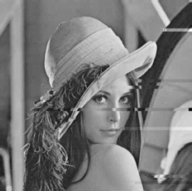
\includegraphics[width=0.42\linewidth]{images/LenaDamaged.png}}
		\subfloat[Détection de la détérioration (blocs noirs)]{
			\label{fig-LenaDetected}
			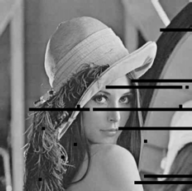
\includegraphics[width=0.42\linewidth]{images/LenaDetected.png}}
	}
	\caption[Résultat de la détection d'erreurs avec les mesures de
\citeauthor{Ye2003}]{Exemple du résultat de la détection d'erreurs avec les mesures de
\citeauthor{Ye2003}. \\Tirée de \citet[p.~371]{Ye2003}}
	\label{fig-LenaYe}
\end{figure}

La détérioration visuelle observée dans l'image de la \fig{fig-LenaDamaged}
résulte d'un taux d'erreurs binaires de $3\times 10^{-4}$. Avec ce taux,
\citet{Ye2003} observent des gains de PSNR allant de 5 à 10 dB selon l'image,
l'emplacement de la détérioration visuelle et le type d'approche de
dissimulation d'erreurs utilisée (l'interpolation linéaire, l'interpolation
directionnelle ou par prédiction des coefficients DCT).

\end{section}

\begin{section}{L'amélioration des approches d'analyse syntaxique d'encodage
vidéo}
\label{sect-SyntaxeAnalysis}
Dans le but d'améliorer l'efficacité des règles de validation de syntaxe de la
norme MPEG-4 Visual présentées par \citet{Talluri1998}, \citeauthor{Yan2003}
proposent une nouvelle règle de validation qui augmente considérablement
l'efficacité de ce genre d'approche. Cette règle permet de valider, entre deux
marqueurs de synchronisation, que le nombre de COD soit égal au nombre de blocs
\citep{Yan2003}. Voici le raisonnement derrière cette approche. Tout
d'abord, les marqueurs de synchronisation sont des séquences binaires uniques
qui servent de point de repère pour le décodeur. Le COD est un bit positionné en
début de macrobloc, qui identifie si ce dernier est encodé ou pas. Le nombre de
macroblocs contenus dans une tranche est disponible dans les paramètres
d'encodages. S'il y a eu désynchronisation, ces deux nombres risquent d'être
différents. Pour des séquences QCIF, encodées à 96 kb/s, \citet{Yan2003}
affirment que leur approche est capable de détecter entre 90\% et 100\% des
erreurs binaires, selon la séquence et le taux d'erreurs binaires utilisés
(allant de 0.2\% à 1.0\%).

Toujours dans le même ordre d'idée, en \citeyear{Superiori2006},
\citeauthor{Superiori2006} proposent un valideur de syntaxe H.264. Ce valideur
identifie des séquences de codes binaires invalides engendrées par la
désynchronisation des codes entropiques, suite à une erreur
\citep{Superiori2006}. Ce valideur est exhaustif et définit des restrictions sur
les valeurs d'un grand nombre de paramètres de la norme.


\citeauthor{Superiori2006} proposent trois catégories d'erreurs de
décodage selon les caractéristiques de l'erreur~\citep{Superiori2006}~:
\begin{description}
 	\item[\bul Code numérique invalide:] Il s'agit ici d'un code
 	qui n'est pas dans la table de codes numériques associés à ce paramètre.
 	\item[\bul Code hors de portée:] Cette erreur survient lorsqu'une valeur
 	décodée est à l'extérieur de l'ensemble des valeurs valides pour le paramètre en question.
 	\item[\bul Erreur contextuelle:] Cette erreur survient si le
 	décodeur doit effectuer une opération invalide.
\end{description}

Les tests de \citeauthor{Superiori2006} ont été effectués sur la séquence QCIF
\textit{Foreman} encodée avec un QP fixé à 28. Dans ces conditions, leur
approche réussit à détecter 60~\% des erreurs binaires provenant de trames
corrompues intra et 47~\% de celles provenant de trames inter, selon
\citep{Superiori2006}.
\end{section}

\begin{section}{La combinaison de l'analyse syntaxique et de la
détection de la détérioration visuelle dans le domaine des pixels}
\label{sect-Combined}
En \citeyear{Superiori2007}, \citeauthor{Superiori2007} combinent leur approche
de validation syntaxique à un algorithme d'identification de la détérioration
visuelle inspiré de \citet{Ye2003}, et auquel un système de vote a été ajouté,
afin d'améliorer le résultat de la détection \citep{Superiori2007}. Dans son
mémoire, \citeauthor{Ikuno2007}q explique en détail l'algorithme proposé
\citep{Ikuno2007}.

La détection de la détérioration visuelle est réalisée dans le domaine des
pixels. Pour isoler l'erreur, \citeauthor{Superiori2007} utilisent le
différentiel de la trame à évaluer par rapport à celle qui la précède (c.-à-d.
la différence entre ces deux trames). La figure~\ref{fig-IkunoForeman} montre
une trame endommagée ainsi que la trame qui la précède. Le différentiel entre
ces deux images est calculé en effectuant une différence absolue entre les
pixels correspondants (même position spatiale). Le résultat du différentiel des
images de la figure~\ref{fig-IkunoForeman} est présenté à la
figure~\ref{fig-IkunoDiff}.

\begin{figure}
	\fbox{\centering
		\subfloat[Trame endommagée]{
			\label{fig-IkunoBroken}
			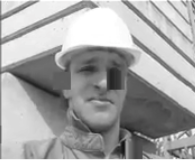
\includegraphics[width=0.42\linewidth]{images/IkunoBroken.png}}
		\subfloat[Trame précédente]{
			\label{fig-IkunoPrev}
			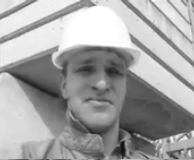
\includegraphics[width=0.42\linewidth]{images/IkunoPrev.png}}
	}
	\caption[Trames utilisées par \citeauthor{Ikuno2007} pour son algorithme
détection]{Trames utilisées par \citeauthor{Ikuno2007} pour démontrer
l'algorithme de détection de la détérioration visuelle. Tirée de
\citet[p.~25]{Ikuno2007}}
	\label{fig-IkunoForeman}
\end{figure}

Par la suite, les valeurs du différentiel sont regroupées en blocs $8 \times 8$
et la moyenne est assignée comme étant représentative de l'énergie du bloc
\citep[p.~27-28]{Ikuno2007}, comme illustré à la \fig{fig-IkunoDiffAnalysis}.
Les erreurs détectées à la \fig{fig-IkunoDiffDetection} sont obtenues à l'aide d'un
seuil. Si la valeur de l'énergie d'un bloc est supérieure à ce seuil, le
bloc est considéré comme erroné.

\begin{figure}
	\fbox{\centering
		\subfloat[Différentiel]{
			\label{fig-IkunoDiff}
			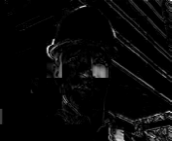
\includegraphics[width=0.30\linewidth]{images/FrameDifference.png}}
		\subfloat[Analyse du différentiel]{
			\label{fig-IkunoDiffAnalysis}
			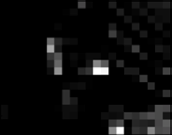
\includegraphics[width=0.30\linewidth]{images/FrameDifferenceAnalysis.png}}
		\subfloat[Erreurs détectées]{
			\label{fig-IkunoDiffDetection}
			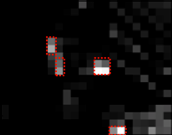
\includegraphics[width=0.30\linewidth]{images/FrameDifferenceDetection.png}}
	}
	\caption[Exemple de l'analyse et de la détection d'erreurs]{Exemple de l'analyse et de la détection d'erreurs.
\\Tirée de \citet[p.~25]{Ikuno2007}}
	\label{fig-FrameDiff}
\end{figure}

De plus, la détection d'effets de bloc en bordure de blocs est effectuée. Pour
trouver les bordures à l'intérieur des trames, les composantes
horizontales~\ref{fig-HaarVert} et verticales~\ref{fig-HaarHori}, d'un filtre de
Haar \citep{Haar1911}, sont combinées et seulement les valeurs en bordure de
blocs sont conservées~\ref{fig-HaarCombined}. L'analyse des effets de bloc est
accomplie pour les blocs $8 \times 8$ et pour les macroblocs $16 \times 16$.
Ceux-ci sont comparés à des seuils, afin de savoir s'il y a présence d'erreurs.

\begin{figure}
	\fbox{\centering
		\minibox{
			\subfloat[Composante verticale]{
				\label{fig-HaarVert}
				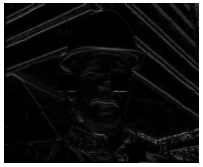
\includegraphics[width=0.40\linewidth]{images/Haar_Vert.png}}
			\subfloat[Composante horizontale]{
				\label{fig-HaarHori}
				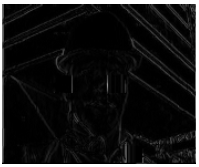
\includegraphics[width=0.40\linewidth]{images/Haar_Hori.png}}\\ %
			\subfloat[Combinaison des deux composantes]{
				\label{fig-HaarCombined}
				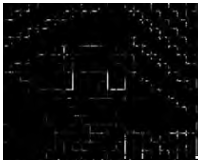
\includegraphics[width=0.40\linewidth]{images/Haar_Combined.png}}
			\subfloat[Analyse de bodures de blocs]{
				\label{fig-HaarAnalysed}
				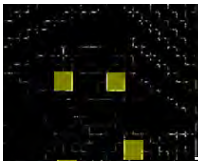
\includegraphics[width=0.40\linewidth]{images/Haar_Analysed.png}}
		}
	}
	\caption[Composantes et analyse du filtre de Haar]{Composantes et analyse du
filtre de Haar. \\Tirée de \citet[p.~26]{Ikuno2007}}
	\label{fig-Haar}
\end{figure}

Les mesures d'énergie et d'effets de bloc sont interprétées par un système de
vote qui détermine où se trouvent les blocs erronés à l'intérieur de la trame
évaluée. Selon \citet{Superiori2007}, l'approche proposée améliore de 1.36~dB,
en moyenne, de PSNR des trames de la séquence QCIF \textit{foreman}. Celles-ci
sont encodées avec un QP fixé à 28 et sont exposées à un taux d'erreurs de
$10^{-5}$. Ce résultat est obtenu par la moyenne des résultats de l'exécution de
20 simulations.

L'année suivante, \citeauthor{Farrugia2008} reprennent les travaux de
\citet{Superiori2007} et retirent les seuils et le système de vote. Ceux-ci sont 
remplacés par une machine à vecteurs de support \citep{SVM1995}. Cette dernière
est une méthode d'apprentissage supervisée qui, une fois entrainée sur un
ensemble de données, est capable de classifier d'autres données. Pour ce genre
d'algorithme, le temps d'entrainement est long, mais la classification est très
rapide, ce qui en fait un bon choix pour des considérations \textit{temps réel}
\citep{Farrugia2008}.

Le vecteur d'entrée (\textit{feature vector}) définit par
\citeauthor{Farrugia2008} possède huit composantes: \begin{enumerate}[$\quad$1.]
  \item AIDB; \item La moyenne du $\text{IAIDB}_{block}$; \item L'écart type du
  $\text{IAIDB}_{block}$; \item IAIDB vertical; \item IAIDB horizontal; \item La
  moyenne du AIDSB; \item L'écart type du AIDSB; \item TC.
\end{enumerate}

\vspace{2em}

\begin{figure}
	\fbox{\centering
		\subfloat[AIDB / $\text{IAIDB}_{block}$]{
			\label{fig-DebonoAIDB}
			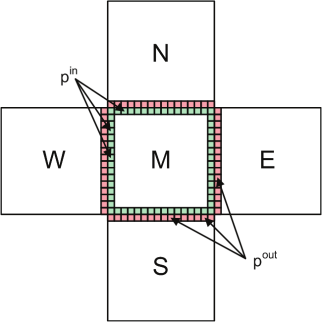
\includegraphics[width=0.30\linewidth]{images/DebonoAIDB.png}}
		\hspace{0.4em}
		\subfloat[IAIDB]{
			\label{fig-DebonoIAIDB}
			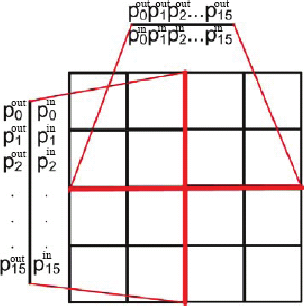
\includegraphics[width=0.30\linewidth]{images/DebonoIAIDB.png}}
		\hspace{0.4em}
		\subfloat[AIDSB]{
			\label{fig-DebonoAIDSB}
			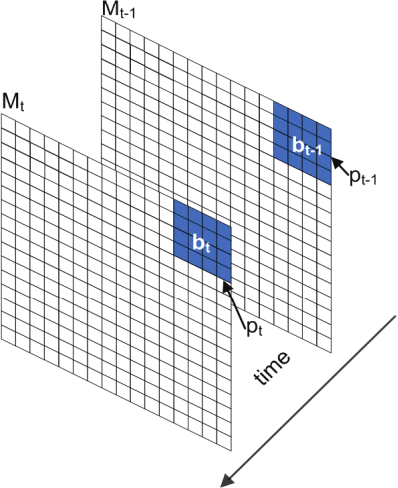
\includegraphics[width=0.30\linewidth]{images/DebonoIAIDSB.png}}
	}
	\caption[Visualisation des composantes du vecteur d'entrée]
	{Visualisation des composantes du vecteur d'entrée. \\Tirée de \citet[p.~79-80]{Farrugia2010}}
	\label{fig-Debono}
\end{figure}

Ce vecteur représente un macrobloc contenu à l'intérieur d'une trame d'une
séquence vidéo. Le AIDB est la différence moyenne des pixels en bordure de
macroblocs (M, à la \fig{fig-DebonoAIDB}). Le $\text{IAIDB}_{block}$ est la même
mesure que le AIDB, mais appliquée aux blocs $4 \times 4$ à l'intérieur d'un
macrobloc. Le IAIDB est la moyenne de la différence des pixels pour les bordures
internes (verticales et horizontales) d'un macrobloc (lignes rouges
\fig{fig-DebonoIAIDB}). Le AIDSB est l'énergie d'un macrobloc $16 \times 16$,
tel que défini par \citet{Ikuno2007}, soit la moyenne du différentiel par
rapport à la trame précédente (voir la \fig{fig-DebonoAIDSB}). La consistance de
la texture (TC) est basée sur une approche d'analyse de texture présentée par
\citet{Wang1990}, connue sous le nom de patron binaire local \ang{Local Binary
Pattern (LBP)}.

\citeauthor{Farrugia2008} ont effectué des tests avec des observateurs humains
pour déterminer l'importance de la détérioration visuelle. Par la suite, ils
utilisent cette information pour mesurer leur solution. Celle-ci identifie en
moyenne 95.25\% des détériorations qu'ils ont qualifiées de \textit{Very
Annoying}, \textit{Annoying} et \textit{Slightly Annoying}. Pour la
détérioration visuelle qu'ils qualifient de \textit{Perceptible but not
Annoying} le taux de détection est de 62.91\%. Les séquences utilisées sont de
résolution QCIF, encodées à 128 kb/s.

\end{section}

En somme, ce chapitre offre un bref survol des travaux de recherche en lien
avec le \textit{Joint Source Channel Decoding}, la résilience aux erreurs lors
du transport de vidéo, la validation de syntaxe pour les normes d'encodage vidéo
et la détection de la détérioration visuelle dans le domaine des pixels. Ces
concepts sont présentés dans un ordre quasi chronologique, où la cohésion
conceptuelle a raison de la chronologie. Conséquemment, ils servent
de notions fondatrices aux approches proposées dans cet ouvrage et présentées
dans le prochain chapitre.